\icode{E-MD-CA-L3-261112-009}
如图，质量 \(m_B=\) \,\qty{1}{kg}的木板\(B\)，静止在粗糙的水平地面上，其水平上表面左端静置一个质量 \(m_A =\) \,\qty{3}{kg}的小滑块（可视为质点），小滑块与板间的动摩擦因数 \(\mu_1 = 0.4\)，木板与地面间的动摩擦因数\(\mu_2 = 0.1\)。从某时刻开始，用水平力 \(F\)直向右拉木板，\(g\) 取\qty{10}{m/s^2}。求：
\begin{enumerate}
	\item 若\(F =\) \,\qty{3}{N}，在施加力\(F\)瞬间，滑块的加速度\(a_1\)和木板的加速度\(a_2\)；
	\item 若\(F =\) \,\qty{24}{N}，在施加力\(F\)瞬间，滑块的加速度\(a_1\)和木板的加速度\(a_2\)；
	\item 若\(F =\) \,\qty{36}{N}，在施加力\(F\)瞬间，滑块的加速度\(a_1\)和木板的加速度\(a_2\)；
\end{enumerate}

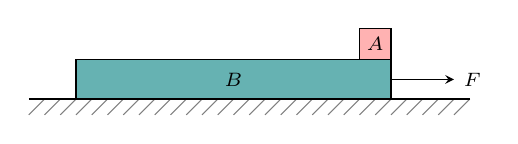
\begin{tikzpicture}[>=stealth,font=\scriptsize]
	\draw[fill=teal!60] (0,0) rectangle(4,.5)node[midway]{\(B\)};
	\draw[fill=red!30] (3.6,.5) rectangle(4,.9)node[midway]{\(A\)};
	\draw[->] (4,.25)--++(.8,0)node[right]{\(F\)};
	\foreach \x in {-.6,-.4,...,5}
		\draw[gray] (\x,-.2)--++(.2,.2);
	\draw[thick] (-.6,0)--(5,0);
\end{tikzpicture}
\begin{answer}
    
\end{answer}